% The report-class-based template was created by R. Jacob Vogelstein in May, 2007
% Updated by Noah J. Cowan on March 1, 2010
% Updated by Brian D. Weitzner on April 29, 2014 
% Updated by John Muschelli on January 29, 2016 
% Updated by Leonardo Collado Torres on April 13, 2016 
% Updated by John Clayton in December, 2019
% Updated by Bibekananda Datta in February, 2024


\documentclass[12pt]{report}


%%%%%%%%%%%%%%%% JH Library-specific settings for PDF/A %%%%%%%%%%%%%%%%%
% PDF Creation settings (required for JH library)
\pdfcompresslevel=9
\pdfminorversion=5
\pdfobjcompresslevel=2

% Needed to create a PDF/A file
\usepackage[a-1b]{pdfx}
\usepackage{pdfpages}
\usepackage{pax}
%%%%%%%%%%%%%%%% JH Library-specific settings for PDF/A %%%%%%%%%%%%%%%%%



%%%%%%%%%%%%%%%%%%%%%%%%%%%%% LaTeX Packages %%%%%%%%%%%%%%%%%%%%%%%%%%%%

%% add more packages as you need (remember sometimes the order of the package matters)
\usepackage[utf8]{inputenc}	    %input
\DeclareUnicodeCharacter{2212}{-}


% math packages
\usepackage{amsfonts,amssymb,amsmath,amsthm,dsfont,mathtools,mathbbol,siunitx,upgreek,mathrsfs,cancel}
\allowdisplaybreaks[1]
\usepackage{autobreak}
\usepackage[ruled]{algorithm2e} %algorithm package
\usepackage[titletoc]{appendix}

\usepackage[american]{babel}
\usepackage[natbib, backend=biber, style=apa, doi=true]{biblatex}
\usepackage{blindtext}

\usepackage{calc}
\usepackage[font=small, labelfont=bf, labelsep=period,  hypcap=true]{caption}
\usepackage{color}
\usepackage{epigraph,varwidth}
\usepackage{enumitem}			%list environment
\usepackage{float}
\usepackage[T1]{fontenc}
\usepackage{graphicx}


\usepackage{geometry}
\usepackage{fancyhdr}
\usepackage[pdfa]{hyperref}
\usepackage[all]{hypcap}
% For captions on the side of figures
\usepackage{ifthen}
\usepackage{lscape}
\usepackage{lipsum}
\usepackage[pagewise,mathlines]{lineno}     % linenumbers
\usepackage{csquotes}                       % for quote environment


\usepackage{listings}
\lstset{basicstyle=\footnotesize\ttfamily,columns=flexible,breaklines=true}
% table related packages
\usepackage{booktabs,longtable,makecell,multicol,multirow,tabularx,xltabular}
%\usepackage[protrusion]{microtype}
\usepackage{textcomp}
\usepackage{sectsty}

\usepackage{setspace}
\usepackage{seqsplit}
\usepackage[rightcaption]{sidecap}
\usepackage{soul}
\usepackage[titles]{tocloft}
\usepackage{parskip}
\usepackage{titlesec}
%\usepackage{tocbibind}
\usepackage{tikz}
\usetikzlibrary{positioning}
\usetikzlibrary{shapes,arrows}
\usepackage{subfig}    % Individual panel captions
\usepackage{xcolor}

%% add more packages as you need

%%%%%%%%%%%%%%%%%%%%%%%%%% END LaTeX Packages %%%%%%%%%%%%%%%%%%%%%%%%%%%




%%%%%%%%%%%%%%%%%%%%%%%%%%%% SETTINGS FOR TOC %%%%%%%%%%%%%%%%%%%%%%%%%%%

%%%% TOC shows 3 levels (chapter to subsection) in the list
\setcounter{tocdepth}{3}
\setcounter{secnumdepth}{3}     % section to ... subsubsection


% Dots for chapters too
\renewcommand{\cftchapleader}{\cftdotfill{\cftdotsep}}


% Tweak to TOC to add 'chapter' to the chapter name instead of a number only
% Set the width of the box based on the longest label name
\renewcommand{\cftchappresnum}{\chaptername\space}
\setlength{\cftchapnumwidth}{\widthof{\textbf{Appendix~999~}}}


% Tweak to TOC to add 'Figure' to the figure caption listing
% To change the distance to the start of the figure title
\renewcommand{\cftfigpresnum}{\bfseries Figure }
\setlength{\cftfignumwidth}{\widthof{\textbf{Figure~99.999~}}}

% Tweak to TOC to add 'Table' to the Table caption listing
% To change the distance to the start of the figure title
\renewcommand{\cfttabpresnum}{\bfseries Table }
\setlength{\cfttabnumwidth}{\widthof{\textbf{Table~99.100~}}}


%%%% UNNUMBERED CHAPTERS, SECTION, and SUBSECTION COMMAND for ADDING to TOC
% Removes 'Chapter #' title while keeping
% it listed in the TOC
\newcommand\chap[1]{%
  \chapter*{#1}%
  \addcontentsline{toc}{chapter}{#1}}
% Removes 'Section #' title while keeping
% it listed in the TOC
\newcommand\sect[1]{%
  \section*{#1}%
  \addcontentsline{toc}{section}{#1}}
% Removes 'Subsection #'title while keeping
% it listed in the TOC
\newcommand\subsect[1]{%
  \subsection*{#1}%
  \addcontentsline{toc}{subsection}{#1}}

%%%%%%%%%%%%%%%%%%%%%%%%%% END SETTINGS FOR TOC %%%%%%%%%%%%%%%%%%%%%%%%%




%%%%%%%%%%%%%%%%%%%% SETTINGS FOR CHAPTER HEADINGS %%%%%%%%%%%%%%%%%%%%%%

%% chapter # and title settings (with gaps)
%% if you use an epigraph after the chapter title then perhaps reduce the first \vspace* from 0 pt to -(some_value)
\makeatletter
\def\@makechapterhead#1{%
  \vspace*{0 \p@}            % space from the top of the page to chapter #
  {\parindent \z@ \raggedright \normalfont
    \ifnum \c@secnumdepth >\m@ne
        \singlespacing \Large \bfseries \@chapapp\enskip \thechapter 
        \\ \vspace{-12pt}   % space between chapter # and title
    \fi
        \interlinepenalty\@M
        \singlespacing \Large \bfseries #1\par\nobreak
    \vskip 24 \p@           % space between the chapter title and the following text
  }}
\makeatother


%%%% settings for unnumbered chapters
% if you use an epigraph after the chapter title then perhaps reduce the first \vspace* from 0 pt to - (some_value)
\makeatletter
\def\@makeschapterhead#1{%
  \vspace*{0 \p@}           % space before the title
  {\parindent \z@ \raggedright
    \normalfont
    \interlinepenalty\@M
    \Large \singlespacing \bfseries  #1\par\nobreak
    \vskip 24 \p@ % space after the title
  }}
\makeatother

%%%%%%%%%%%%%%%%%% END SETTINGS FOR CHAPTER HEADINGS %%%%%%%%%%%%%%%%%%%%





%%%%%%%%%%%%%%%%%%%%%%%%%% EPIGRAPH SETTINGS %%%%%%%%%%%%%%%%%%%%%%%%%%%%

% Following settings allow the epigraph and the underline 
% to be arbitrary to the epigraph length
\renewcommand{\epigraphflush}{flushright}
\renewcommand{\epigraphsize}{\small}
\setlength{\epigraphwidth}{0.6\textwidth}
\renewcommand{\textflush}{flushright}
\renewcommand{\sourceflush}{flushright}
% A useful addition
\newcommand{\epitextfont}{\itshape}
\newcommand{\episourcefont}{\scshape}

\makeatletter
\newsavebox{\epi@textbox}
\newsavebox{\epi@sourcebox}
\newlength\epi@finalwidth
\renewcommand{\epigraph}[2]{%
  \vspace{\beforeepigraphskip}
  {\epigraphsize\begin{\epigraphflush}
   \epi@finalwidth=\z@
   \sbox\epi@textbox{%
     \varwidth{\epigraphwidth}
     \begin{\textflush}\epitextfont#1\end{\textflush}
     \endvarwidth
   }%
   \epi@finalwidth=\wd\epi@textbox
   \sbox\epi@sourcebox{%
     \varwidth{\epigraphwidth}
     \begin{\sourceflush}\episourcefont#2\end{\sourceflush}%
     \endvarwidth
   }%
   \ifdim\wd\epi@sourcebox>\epi@finalwidth 
     \epi@finalwidth=\wd\epi@sourcebox
   \fi
   \leavevmode\vbox{
     \hb@xt@\epi@finalwidth{\hfil\box\epi@textbox}
     \vskip 1ex         % gap between quote and rule
     \hrule height \epigraphrule
     \vskip 1ex         % gap between rule and author
     \hb@xt@\epi@finalwidth{\hfil\box\epi@sourcebox}
   }%
   \end{\epigraphflush}
   \vspace{\afterepigraphskip}}}
\makeatother

%%%%%%%%%%%%%%%%%%%%%%%%% END EPIGRAPH SETTINGS %%%%%%%%%%%%%%%%%%%%%%%%%%%




%%%%%%%%%%%%%%%%%%%%%%%%%% DOCUMENT FORMATTING %%%%%%%%%%%%%%%%%%%%%%%%%%%%

%% margin settings required by JH library (geometry package)
\geometry{letterpaper, left=1.5in, right=1.0in, top=1in, bottom=1.0in, includehead, headheight=30pt, headsep=10pt}


%%%% using titlesec package for sections, subsection .. heading format
\titleformat*{\section}{\large\bfseries}
\titleformat*{\subsection}{\normalsize\bfseries}
\titleformat*{\subsubsection}{\normalsize\itshape}


%% settings for paragraph (and not title) spacing, roughly speaking
\renewcommand{\arraystretch}{1.5}       % spacing inside table
\setlength{\parskip}{12pt}              % paragraph skip
\setlength{\parindent}{0pt}             % paragraph indentation
\setlength{\bibitemsep}{\baselineskip}  % bib item separation 


%% settings for hyperref package
\hypersetup{linktocpage, unicode, colorlinks=true, citecolor=blue, filecolor=blue, linkcolor=blue, urlcolor=blue}

%%%%%%%%%%%%%%%%%%%%%%%% END DOCUMENT FORMATTING %%%%%%%%%%%%%%%%%%%%%%%%%





%%%%%%%%%%%%%%%%%%%%%% MATH SETTINGS AND MACROS %%%%%%%%%%%%%%%%%%%%%%%%%

\numberwithin{equation}{chapter}        % eqn no with chapter prefix
\newcommand{\vect}[1]{\mathbf{#1}}
\DeclareMathOperator{\tr}{tr}
\DeclareMathOperator{\divg}{div}
\DeclareMathOperator{\grad}{grad}

%% these are just some examples. add more macros as you need

%%%%%%%%%%%%%%%%%%%%%% MATH SETTINGS AND MACROS %%%%%%%%%%%%%%%%%%%%%%%%%





%%%%%%%%%%%%%%%%%%%%%% SIMPLE COMMENT SETTINGS %%%%%%%%%%%%%%%%%%%%%%%%%%
\newcommand{\COMMENT}{\textcolor{red}}
\newcommand{\ADDCITATION}{\COMMENT{(ADD CITATION)}}
\newcommand{\ADDFIGURE}{\COMMENT{(ADD FIGURE)}}
\newcommand{\ADDTABLE}{\COMMENT{(ADD TABLE)}}

%% you can use some other packages for more complicated review and comment section


%%%%%%%%%%%%%%%%%%%% END SIMPLE COMMENT SETTINGS %%%%%%%%%%%%%%%%%%%%%%%%





%%%%%%%%%%%%%%%%%%%%%%%%%%% BASIC SETTINGS %%%%%%%%%%%%%%%%%%%%%%%%%%%%%%
% add all the images to that folder
% you can add images in chapter-wise PDF format (my preference).
\graphicspath{{figures/}}



%% this file has to be in BibLaTeX format. Use Zotero or some other citation manager to generate the .bib file in BibLaTeX format.
\addbibresource{phd_thesis.bib}



%% choice a font form (or add something else) for your thesis.
\usepackage{lmodern}
%\usepackage[sc]{mathpazo}
%\usepackage{times}             %times new roman

%%%%%%%%%%%%%%%%%%%%%%%%% END BASIC SETTINGS %%%%%%%%%%%%%%%%%%%%%%%%%%%%








%%%%%%%%%%%%%%%%%%%%%%%%% DOCUMENT BEGINS HERE %%%%%%%%%%%%%%%%%%%%%%%%%%
\begin{document}



%%%%%%%%%%%%%%%%%%%%%%%%%%%% FRONT MATTER %%%%%%%%%%%%%%%%%%%%%%%%%%%%%%%%

\onehalfspacing                 % for title page
% JHU Dissertation title page
\thispagestyle{empty}

\begin{center}

{\large \MakeUppercase{\textbf{Lorem ipsum dolor sit amet consectetuer adipiscing elit}}}

\vspace{1in}

by \\
John Doe 
\\ \vspace{1.5in}

A dissertation submitted to The Johns Hopkins University in conformity\\
with the requirements for the degree of Doctor of Philosophy 
\\ \vspace{1in}

Baltimore, Maryland\\       % LOCATION
MONTH YEAR                  % DATE OF SUBMISSION HERE
\\ \vspace{1.5in}

% COPYRIGHT STATEMENT
{\copyright{} YEAR John Doe \\
All rights reserved}

\end{center}
              % title page



% header and page numbering set up
\pagestyle{fancy}
\renewcommand{\chaptermark}[1]{\markboth{#1}{#1}}
\fancyhead[R]{}
\fancyhead[L]{\nouppercase \leftmark}
\pagenumbering{roman}
\setcounter{page}{2}
\doublespacing


% Add abstract, dedication, and acknowledgment
\chap{Abstract} 

%% your abstract goes here (add your abstract)
\Blindtext[3]


%%  committee members go here (do not go to a new page; it should follow the abstract)
\begin{singlespace}

\textbf{Primary reader and thesis advisor:}

Dr. Chuck Darwin \\
Professor\\
Department of Biology\\
Johns Hopkins University, Baltimore MD 

\vspace{0.2in}

\textbf{Secondary readers: }

Dr. Stewart Hawking\\
Professor\\
Department of Biology \\
Johns Hopkins University, Baltimore, MD 

\vspace{0.1in}

Dr.~Jimmy Watson \\
Professor\\
Department of Biology \\
Johns Hopkins University, Baltimore, MD 

\end{singlespace}
\chapter*{~}
\addcontentsline{toc}{chapter}{Dedication}
%% did not use \chap command because the chapter does not have any name

\begin{center}
\vspace*{2in}
    \textit{This thesis is dedicated to ...}
\end{center}

\include{04-acknowledgment}

\onehalfspacing
\renewcommand{\contentsname}{Table of Contents}
\tableofcontents
\listoftables
\addcontentsline{toc}{chapter}{List of Tables}
\listoffigures
\addcontentsline{toc}{chapter}{List of Figures}

%%%%%%%%%%%%%%%%%%%%%%%%%%% END FRONT MATTER %%%%%%%%%%%%%%%%%%%%%%%%%%%%






%%%%%%%%%%%%%%%%%%%%%%%%%%%%%% MAIN TEXT %%%%%%%%%%%%%%%%%%%%%%%%%%%%%%%

\clearpage
\pagenumbering{arabic}
\fancyhead[L]{\chaptername\ \thechapter. \nouppercase \leftmark}
\doublespacing          % restore double spacing in chapter contents


\chapter{Chapter title goes here} \label{chap:chap-1}

\blindtext 
\chapter{Chapter title goes here} \label{chap:chap-2}

% epigraph before chapter heading
\epigraphhead[0]{\epigraph{\enquote{Do not believe everything you see on the internet}}{-- Albert Einstein}}

\blindtext 

\begin{figure}[ht]
\begin{center}
    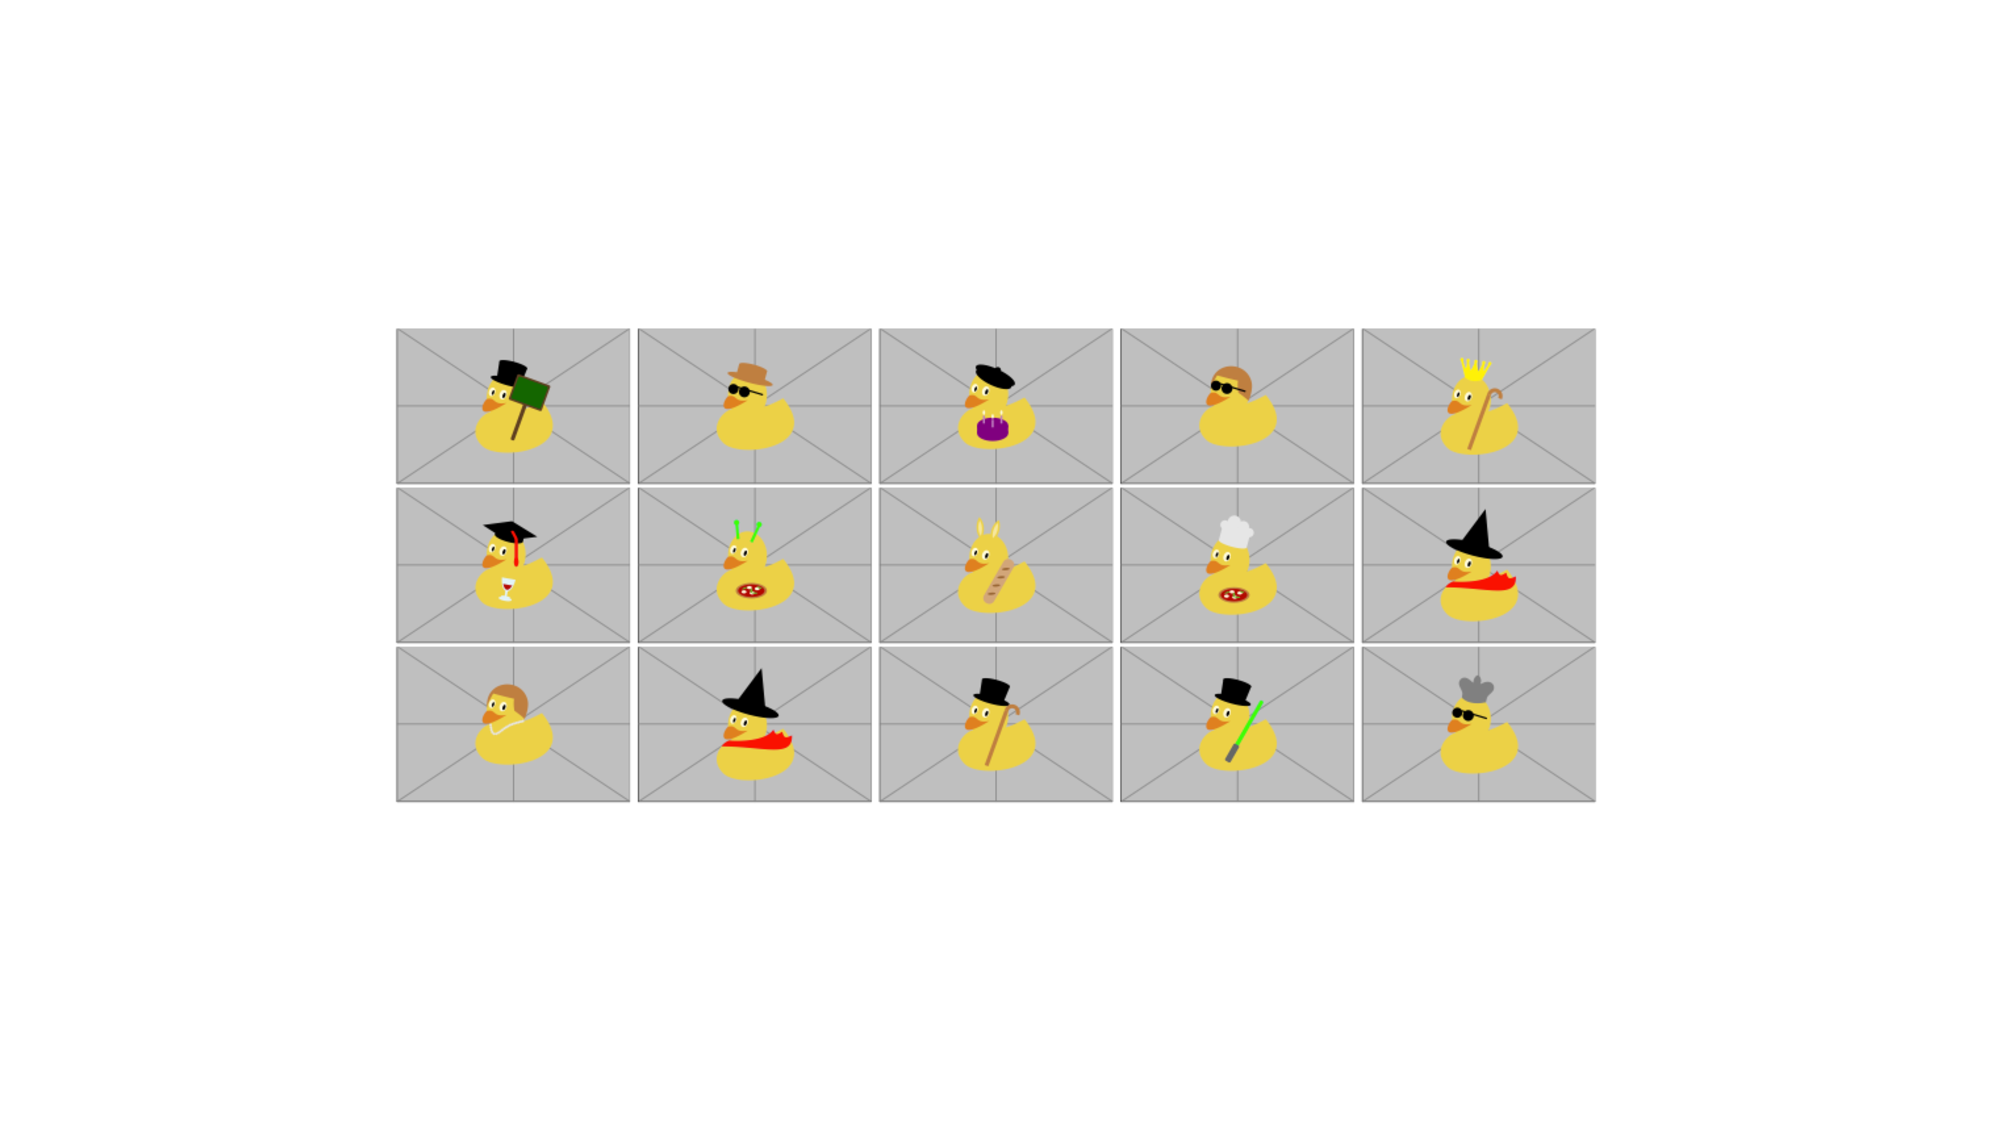
\includegraphics[width=\textwidth, trim={6cm 5cm 6cm 5cm},clip,page=1] {chap2.pdf}
    \caption{Here are some photos of ducks to make you feel happy in tough times.}
    \label{fig:ducks}
\end{center}
\end{figure}

\chapter{Chapter title goes here} \label{chap:chap-3}

% epigraph after chapter heading
\epigraph{\enquote{Since it is written in \LaTeX, it must be true.}}{-- Issac Newton}


\blindtext 
\chapter{Chapter title goes here} \label{chap:chap-4}

% if you want a short header you can use the following command
% \chapter[short-header-name]{chapter-title} \label{chap:chap-4}


% add your chapter text here
\section{Introduction}
\blindtext

\begin{figure}[ht]
\begin{center}
    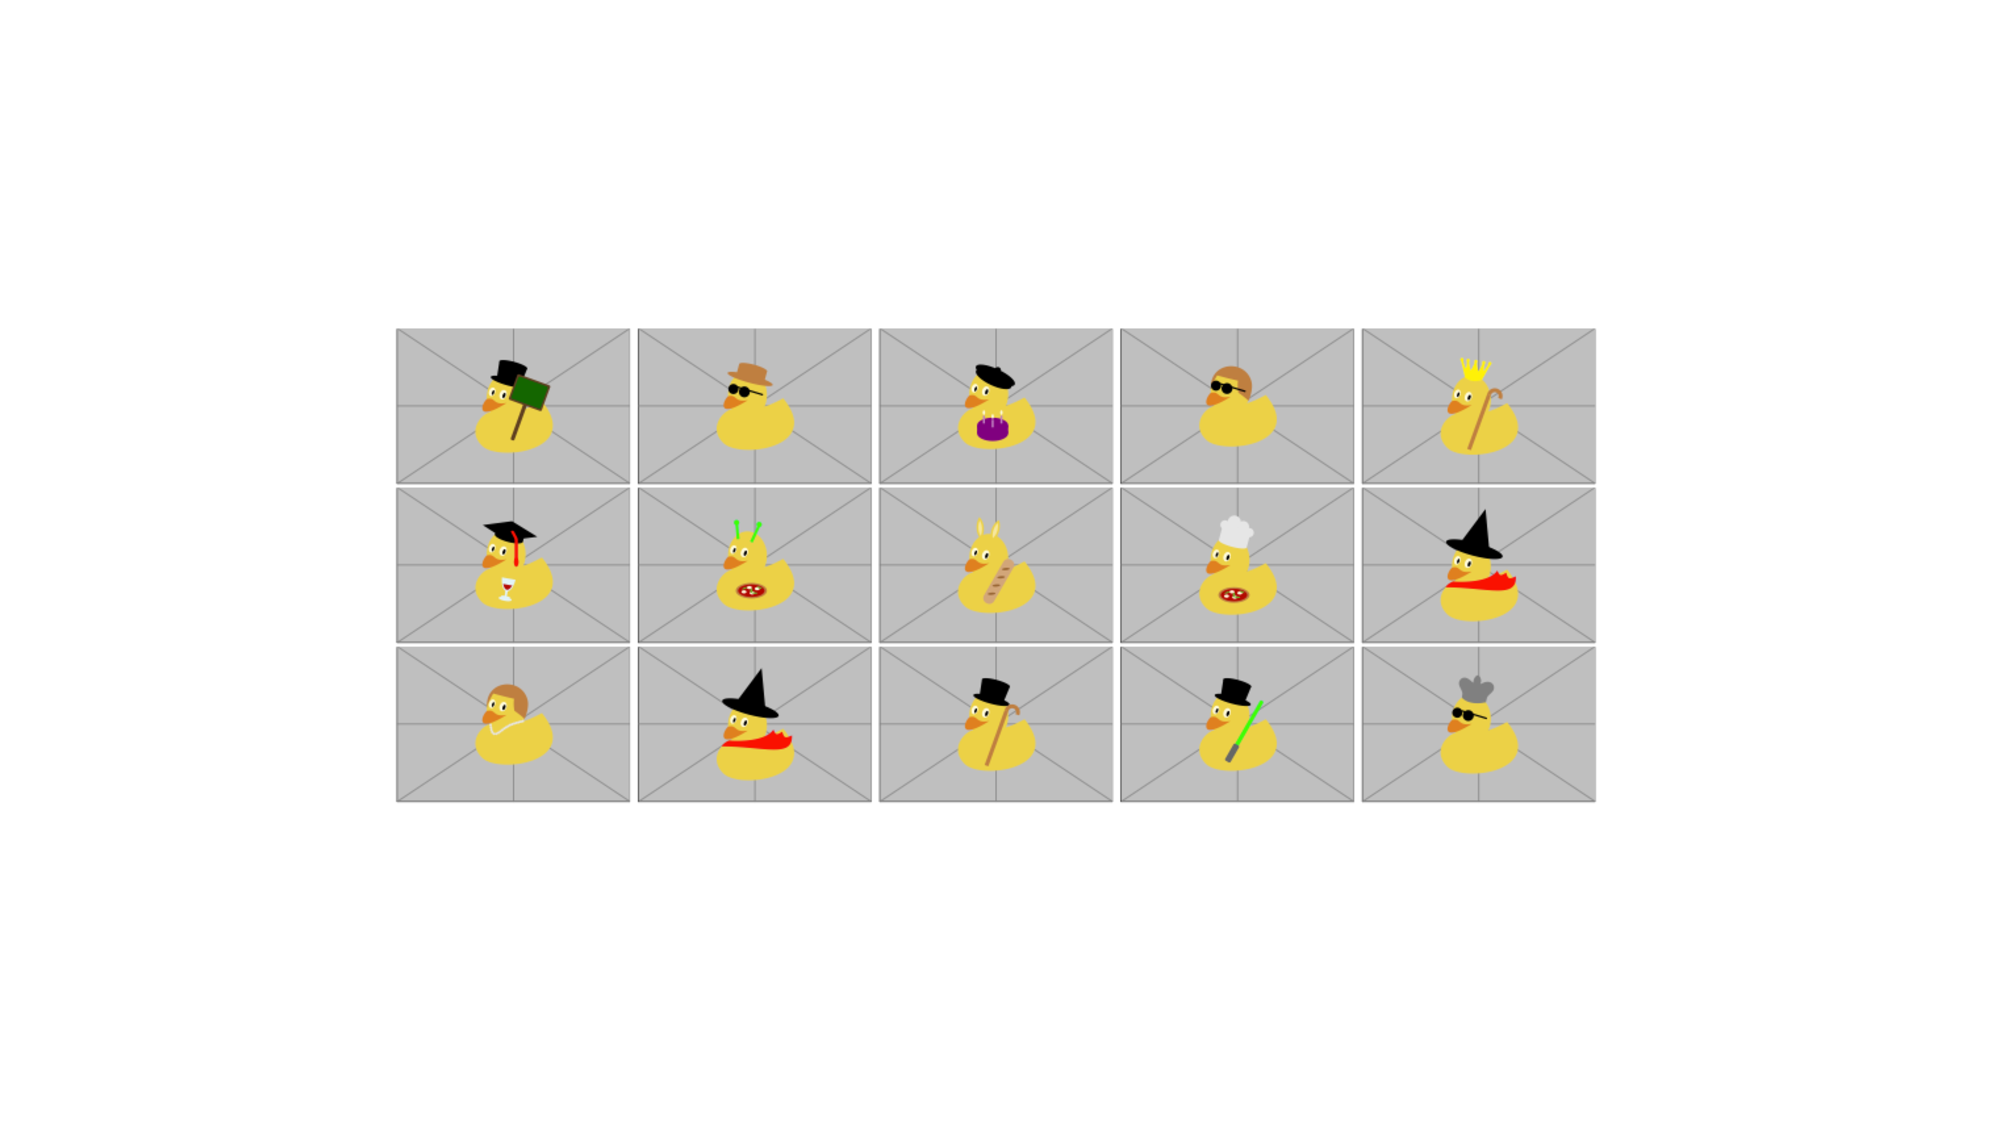
\includegraphics[width=\textwidth, trim={6cm 5cm 6cm 5cm},clip,page=1] {chap2.pdf}
    \caption{Here are some photos of ducks to make you feel happy in tough times.}
    \label{fig:ducks}
\end{center}
\end{figure}


\blindtext[2]
\chapter{Chapter title goes here} \label{chap:chap-5}

% if you want a short header you can use the following command
% \chapter[short-header-name]{chapter-title} \label{chap:chap-5}


% add your chapter text here
\section{Introduction}
\blindtext \parencite{knuth-fa}


%%%%%%%%%%%%%%%%%%%%%%%%%%%% END MAIN TEXT %%%%%%%%%%%%%%%%%%%%%%%%%%%%%




%%%%%%%%%%%%%%%%%%%%%%%%%%%%% BACK MATTER %%%%%%%%%%%%%%%%%%%%%%%%%%%%%%
\clearpage
\singlespacing
\markboth{Bibliographic references}{}
\fancyhead[L]{\leftmark}
\chap{Bibliographic references}


\nocite{*}
\printbibliography[heading=none]


\doublespacing
\fancyhead[L]{\appendixname\ \thechapter. \nouppercase \leftmark}
\appendix 
\makeatletter
\addtocontents{toc}{\protect\renewcommand\protect\cftchappresnum{\@chapapp\ }}
\makeatother
\renewcommand{\thechapter}{\Alph{chapter}}

\chapter{Some necessary information}


\blindtext[5][7]
\chapter{Few more information} \label{chap:appendix-b}

% add your chapter text here
\blindtext

%%%%%%%%%%%%%%%%%%%%%%%%%%% END BACK MATTER %%%%%%%%%%%%%%%%%%%%%%%%%%%%



\end{document}

%%%%%%%%%%%%%%%%%%%%%%%%% DOCUMENT ENDS HERE %%%%%%%%%%%%%%%%%%%%%%%%%%%